\section{Project description and goals}
We plan to use the DeepFashion\cite{liu2016deepfashion} dataset in this project where we train a Deep Neural Network based image ranking system using the triplet margin loss. When a user presents the model with a query image, we hope to retreive top k similar images from the training data and present it to the user. 

Our goals for this project can be briefly summarized as follows :
\begin{itemize}
    \item We have built and trained a model that can efficiently and reliably rank the images
    \item Build a simple GUI that displays the resultant images obtained from our learned model
    \item Additionally we plan to randomly assign a rating to each of these clothing product to emulate the ratings as seen on popular websites like amazon etc. (We are faking the rating by using some random scheme and hence the scores need not make sense). We plan to use these scores to influence the order in which the top "k" results are displayed on the GUI
    \item Since we are currently training and trying to improve the model, we have not yet evaluated the model for the TOP-K-precision metric. However we will be using this (possibly with other metrics like mean average precision) when we are selecting the best model from a candidate set of models.
\end{itemize}



\begin{figure}[tp!]
\centerline{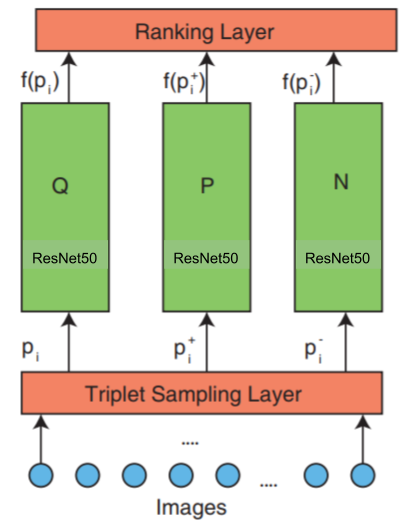
\includegraphics[scale=0.5]{imgs/architecture.png}}
    \caption{Network architecture of Deep Ranking}
    \label{fig:architecture}
\end{figure}






We can see that accuracy will start to saturate at one point and eventually degrade with increase in the number of layers in the deep neural networks. In practise it is seen that shallower networks is much better than deeper counterparts. Resnet uses shortcut connections where one or more layers are skipped to solve the degradation problem. 

\begin{figure}[tp!]
\centerline{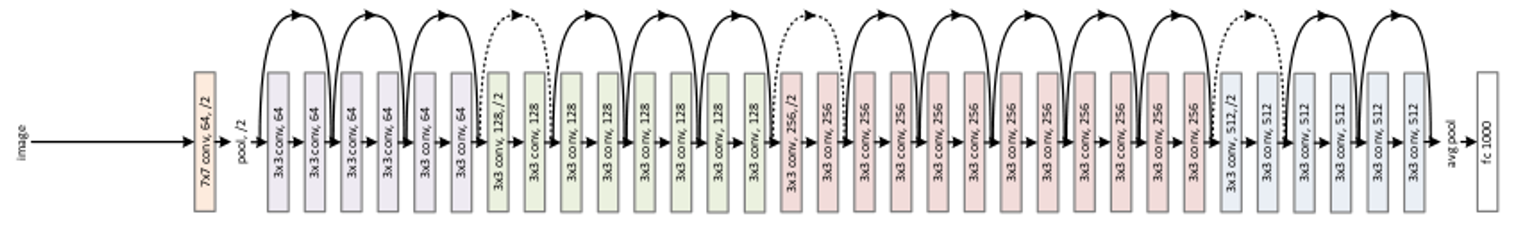
\includegraphics[width=\columnwidth]{imgs/resnet.png}}
    \caption{ResNet architecture}
    \label{fig:resnet}
\end{figure}

We can see from figure \ref{fig:resnet} that ResNet consists of one convolution and one pooling followed by 4 layers of similar behaviour. They perform 3*3 convolution with a fixed map dimension bypassing the input every 2 convolutions. The dotted lines represents a change in the dimension i.e reduction due to convolution. \newline

\begin{flushleft} \textbf{Residual block}
In traditional networks, layers learn the true output (H(x)) where as layer in the residual networks try to learn the residual (R(x)). Let us consider a neutral network block whose input is x and true distribution H(x). We see that \newline
\begin{equation}
    F(x) = Output - Input = H(x) - x 
\end{equation}
Rearranging it, we get
\begin{equation} \label{Output}
    H(x) = F(x) + x
\end{equation}
The layers try to learn the residual, F(x) and the identity connection comes due to x as seen in figure \ref{fig:resnetBlock}. Hence the name \textbf{Residual Block}. \end{flushleft}


% \begin{figure}[tp!]
% \centerline{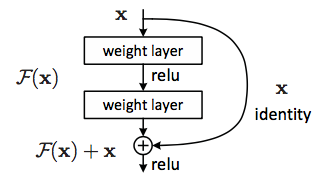
\includegraphics[scale=0.5]{imgs/restnet-block.png}}
%     \caption{Residual learning: building block}
%     \label{fig:resnetBlock}
% \end{figure}
